\chapter{Problem analysis}
\chlab{analysis}

%Problem description and analysis. May be merged with introduction later on...

In this chapter, the problems that this thesis project aims to solve are discussed. First, a brief explanation of the chemical concepts used in the project is provided (\secref{chemical}), followed by the interaction design challenges in \secref{id_challenges}.

\section{Chemical concepts}
\seclab{chemical}
As far as this project is concerned, the most important chemistry knowledge that needs to be present is the fact that every material is built up out of molecules, consisting of a set of atoms. Each atom has its own type, such as hydrogen~(\verb|H|) or carbon~(\verb|C|). The atoms of a molecule are connected in a certain way, where the connections are called bonds. There can be multiple bonds between the same atoms, creating double or triple bonds. Every molecule has a total charge, which is the sum of the charges of the individual atoms in that molecule.

\begin{wrapfigure}{r}{.4\textwidth}
\vspace{-2em}
\begin{center}
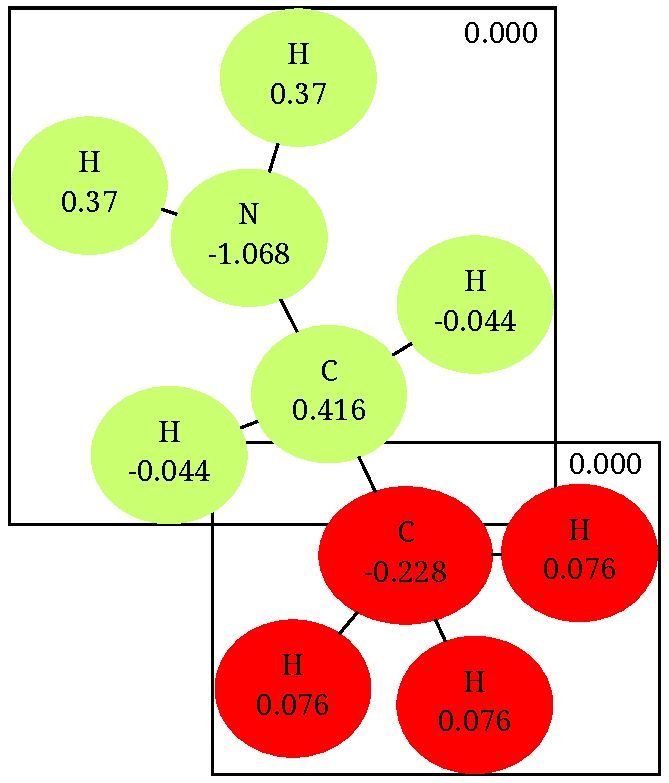
\includegraphics[width=.38\textwidth]{img/ethanamine.pdf}
\caption{Schematic view of ethanamine ($C_{2}H_{7}N$)~\cite{atb2014ethanamine}, including topology data on atom types, atomic charges and charge groups.}
\figlab{partial_charges}
\end{center}
\vspace{-2em}
\end{wrapfigure}

As discussed in the introduction (\chref{introduction}), biomolecular simulations are becoming increasingly important, especially in the field of drug development. For these simulations, force field models are required to describe the interatomic relations of the drug molecules. In order to run a simulation, these force fields require the molecule's topology, which consists of the molecule's atom types, bonds, bond angles, atomic charges and charge groups.

\Figref{partial_charges} shows the schematic view of an ethanamine molecule. Here, every oval symbolises an atom. The atom type is the letter on the top rule of the oval, i.e. \verb|H| is the atom type of the sphere \verb|H7 (6)|. The first number indicates the index in the list of atoms of that type (\verb|7| in the example), the second the overall atom index in the molecule (\verb|6| in the example). The bonds between atoms are shown as lines between the ovals and the atomic charges are given by the number at the bottom row of the oval ($0.37$ for \verb|H7 (6)|). Finally, the colouring of the atoms and the boxes around them denote a charge group. This is a group of connected atoms, for which the total charge is ideally equal to that of the whole molecule ($0.0$ in this example).

In a recent study, El-Kebir, Klau et al. have developed an algorithm that allows for fast and reliable assignment of charge groups~\cite{canzar2012charge}. As this is now optimised, they currently focus on a different step in the parameterisation: that of calculating the atomic partial charges. Currently, these charges are retrieved using complex quantum-mechanical calculations. However, as molecules grow bigger, these calculations can take hours or even days to complete. As it is not believed that these calculations can be speeded up, a different approach is needed for finding atom charges.

As discussed before, a possible approach is to exploit the similarity of molecules, and retrieve the partial charges of an unparameterised molecule from similar fragments in other molecules for which the charges \emph{are} known. In \figref{matching}, the basics of fragment matching are shown. In this case, we are looking for a \verb|C| atom, with three connected \verb|H| atoms (see \figref{match_1}). \Figref{match_2} shows a matching fragment from a different molecule, that, indeed, consists of a \verb|C| with three connected \verb|H|s. The fragment shown in \figref{match_3} obviously does not match with the fragment that is being looked for. It does contain two \verb|H| atoms, but they are connected to an \verb|N| atom, rather than a \verb|C|. More detailed information on fragment matching can be found in \secref{matching}.

\begin{figure}[h!]
\centering
\begin{subfigure}[t]{0.29\textwidth}
\centering
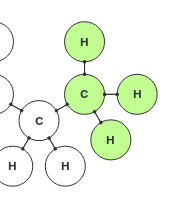
\includegraphics[width=\textwidth]{img/match_1.png}
\caption{Molecule fragment, highlighted in green.}
\figlab{match_1}
\end{subfigure}%
\qquad
\begin{subfigure}[t]{0.29\textwidth}
\centering
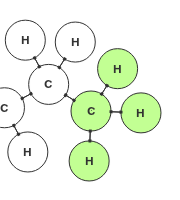
\includegraphics[width=\textwidth]{img/match_2.png}
\caption{Matching fragment, highlighted in green.}
\figlab{match_2}
\end{subfigure}%
\qquad
\begin{subfigure}[t]{0.29\textwidth}
\centering
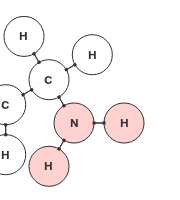
\includegraphics[width=\textwidth]{img/match_3.png}
\caption{Non-matching fragment, highlighted in red / pink.}
\figlab{match_3}
\end{subfigure}
\caption{Basic fragment matching.}
\figlab{matching}
\end{figure}

For an atom or a set of atoms, usually many matching fragments will be found. Which one of those fragments is the best match depends on many factors, including the fragment size and type of molecule they originate from. Due to this, it is currently not possible to fully automate fragment-based paremeterisation. Instead, it needs to be done by experienced chemists who have the knowledge about which fragments match and which do not. A system needs to be developed that assists them in this process, and allows them to easily compare fragments and molecules.


\section{Interaction Design challenges}
\seclab{id_challenges}
\nlipsum



\begin{comment}
 A tool is needed that provides them with a view of the unparameterised molecule and helps them find the best matching fragments. After constructing the charges out of similar fragments, the users should be allowed to manually adjust some values if they feel that this is needed.



Challenges arise here for the interaction design of the tool. It should be possible to easily compare the related fragments, both with each other and with the unparameterised molecule. How to properly do this is still an open question. As there is currently no software that does this, a proper way of comparing molecule fragments needs to be designed from scratch. This allows for really creating something new, but also creates the challenge of doing it right without having any clear starting point.

Next, the tool should encourage its user to compare enough related fragments so that he finds the best match. If, however, there are a lot of related fragments to choose from, the user should be able to easily spot the best ones. Otherwise, it might require too much time to fully parameterise a molecule. This creates another challenge, that of showing a set of related fragments in a clear and intuitive way.

Furthermore, as the molecules that will be analysed vary in size from a few atoms to a few hundred, visualisations of the molecules should be given some thought to make sure both large and small molecules look good. This creates yet another challenge, as it is not trivial to show large atoms on a small screen. A good algorithm should be developed, following which both small and large molecules will be nicely displayed.

Overall, the biggest challenge is to make the tool work intuitively and to implement it such that it makes chemists' work easier. Parameterising a large molecule should therefore not require hours to complete. If it would, using the conventional quantum mechanical calculations would still be preferred, since one can at least do other things while waiting for his results. When one has to manually parameterise a molecule, this is not possible.
\end{comment}
